% GNUPLOT: LaTeX picture with Postscript
\begingroup
\newcommand{\ft}[0]{\footnotesize}
  \makeatletter
  \providecommand\color[2][]{%
    \GenericError{(gnuplot) \space\space\space\@spaces}{%
      Package color not loaded in conjunction with
      terminal option `colourtext'%
    }{See the gnuplot documentation for explanation.%
    }{Either use 'blacktext' in gnuplot or load the package
      color.sty in LaTeX.}%
    \renewcommand\color[2][]{}%
  }%
  \providecommand\includegraphics[2][]{%
    \GenericError{(gnuplot) \space\space\space\@spaces}{%
      Package graphicx or graphics not loaded%
    }{See the gnuplot documentation for explanation.%
    }{The gnuplot epslatex terminal needs graphicx.sty or graphics.sty.}%
    \renewcommand\includegraphics[2][]{}%
  }%
  \providecommand\rotatebox[2]{#2}%
  \@ifundefined{ifGPcolor}{%
    \newif\ifGPcolor
    \GPcolortrue
  }{}%
  \@ifundefined{ifGPblacktext}{%
    \newif\ifGPblacktext
    \GPblacktexttrue
  }{}%
  % define a \g@addto@macro without @ in the name:
  \let\gplgaddtomacro\g@addto@macro
  % define empty templates for all commands taking text:
  \gdef\gplbacktext{}%
  \gdef\gplfronttext{}%
  \makeatother
  \ifGPblacktext
    % no textcolor at all
    \def\colorrgb#1{}%
    \def\colorgray#1{}%
  \else
    % gray or color?
    \ifGPcolor
      \def\colorrgb#1{\color[rgb]{#1}}%
      \def\colorgray#1{\color[gray]{#1}}%
      \expandafter\def\csname LTw\endcsname{\color{white}}%
      \expandafter\def\csname LTb\endcsname{\color{black}}%
      \expandafter\def\csname LTa\endcsname{\color{black}}%
      \expandafter\def\csname LT0\endcsname{\color[rgb]{1,0,0}}%
      \expandafter\def\csname LT1\endcsname{\color[rgb]{0,1,0}}%
      \expandafter\def\csname LT2\endcsname{\color[rgb]{0,0,1}}%
      \expandafter\def\csname LT3\endcsname{\color[rgb]{1,0,1}}%
      \expandafter\def\csname LT4\endcsname{\color[rgb]{0,1,1}}%
      \expandafter\def\csname LT5\endcsname{\color[rgb]{1,1,0}}%
      \expandafter\def\csname LT6\endcsname{\color[rgb]{0,0,0}}%
      \expandafter\def\csname LT7\endcsname{\color[rgb]{1,0.3,0}}%
      \expandafter\def\csname LT8\endcsname{\color[rgb]{0.5,0.5,0.5}}%
    \else
      % gray
      \def\colorrgb#1{\color{black}}%
      \def\colorgray#1{\color[gray]{#1}}%
      \expandafter\def\csname LTw\endcsname{\color{white}}%
      \expandafter\def\csname LTb\endcsname{\color{black}}%
      \expandafter\def\csname LTa\endcsname{\color{black}}%
      \expandafter\def\csname LT0\endcsname{\color{black}}%
      \expandafter\def\csname LT1\endcsname{\color{black}}%
      \expandafter\def\csname LT2\endcsname{\color{black}}%
      \expandafter\def\csname LT3\endcsname{\color{black}}%
      \expandafter\def\csname LT4\endcsname{\color{black}}%
      \expandafter\def\csname LT5\endcsname{\color{black}}%
      \expandafter\def\csname LT6\endcsname{\color{black}}%
      \expandafter\def\csname LT7\endcsname{\color{black}}%
      \expandafter\def\csname LT8\endcsname{\color{black}}%
    \fi
  \fi
  \setlength{\unitlength}{0.0500bp}%
  \begin{picture}(7200.00,5040.00)%
    \gplgaddtomacro\gplbacktext{%
      \csname LTb\endcsname%
      \put(1210,820){\makebox(0,0)[r]{\strut{} 1e+27}}%
      \put(1210,1272){\makebox(0,0)[r]{\strut{} 1e+28}}%
      \put(1210,1724){\makebox(0,0)[r]{\strut{} 1e+29}}%
      \put(1210,2177){\makebox(0,0)[r]{\strut{} 1e+30}}%
      \put(1210,2629){\makebox(0,0)[r]{\strut{} 1e+31}}%
      \put(1210,3081){\makebox(0,0)[r]{\strut{} 1e+32}}%
      \put(1210,3534){\makebox(0,0)[r]{\strut{} 1e+33}}%
      \put(1210,3986){\makebox(0,0)[r]{\strut{} 1e+34}}%
      \put(1210,4438){\makebox(0,0)[r]{\strut{} 1e+35}}%
      \put(1571,484){\makebox(0,0){\strut{} 1e+11}}%
      \put(2663,484){\makebox(0,0){\strut{} 1e+12}}%
      \put(3755,484){\makebox(0,0){\strut{} 1e+13}}%
      \put(4847,484){\makebox(0,0){\strut{} 1e+14}}%
      \put(5939,484){\makebox(0,0){\strut{} 1e+15}}%
      \put(176,2739){\rotatebox{-270}{\makebox(0,0){\strut{}Pressure (barye)}}}%
      \put(4072,154){\makebox(0,0){\strut{}Density (g/cm$^3$)}}%
    }%
    \gplgaddtomacro\gplfronttext{%
      \csname LTb\endcsname%
      \put(2329,4602){\makebox(0,0)[l]{\strut{}Hempel DD2}}%
      \csname LTb\endcsname%
      \put(2329,4382){\makebox(0,0)[l]{\strut{}G. Shen FSU 2.1}}%
      \csname LTb\endcsname%
      \put(2329,4162){\makebox(0,0)[l]{\strut{}SFHo}}%
      \csname LTb\endcsname%
      \put(2329,3942){\makebox(0,0)[l]{\strut{}SFHx}}%
      \csname LTb\endcsname%
      \put(2329,3722){\makebox(0,0)[l]{\strut{}LS220}}%
    }%
    \gplbacktext
    \put(0,0){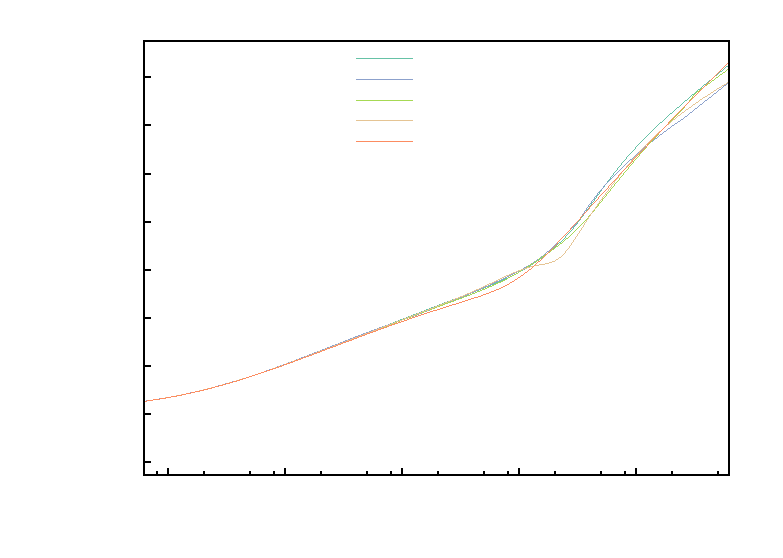
\includegraphics{images/pressure-vs-density-T10-Ye0.05}}%
    \gplfronttext
  \end{picture}%
\endgroup
